% !TeX root = ../document_maitre.tex

La facilité d'usage d'un \gls{sgc} n'est pas le seul frein rencontré. Face à la complexification de gestion de certaine typologie, ces logiciels atteignent leurs limites. C'est le cas de l'\gls{imgani} dont la description et la gestion sont éminement complexe.\footnote{Voir \fullref{imageAnimee}}.

Les \glspl{sgc} rencontrent aujourd'hui des limites particulières à la gestion de cet objet. À l'image de S-Movies, l'indexation et le stockage de segments vidéos liés à des notices \gls{WEMI} ne rencontrent pas de frein particulier. Mais l'absence de moyen de traitement et d'indexation automatisée directement intégré à l'application constitue un frein. 

Les besoins descriptifs et la réalité de conservation de cet objet font de l'absence d'un module de traitement dédié une limite d'usage.\footnote{\fullref{imganiExemple}}. 

Alors disposer d'un outil d'indexation semi-automatisée devient un objectif. Cependant, les tentatives d'indexation semi-automatisée ou automatisée de l'\gls{imgani} sont aujourd'hui en demi-teinte. Il existe certaines solutions propriétaires, assez peu convaincante dans un usage patrimonial. Et pour l'\gls{ops}, il n'existe qu'une myriade d'outils traitant de points spécifiques.\footnote{\fullref{réalitéIndexationAuto}}\newline

Notons que cet outil fait face à ces propres enjeux bien différents de ceux soulevés par les précédents outils.

Pour l'indexation semi-automatisée des \glspl{imgani}, il s'agit bien de produire de la donnée scientifique afin d'indexer les collections. On touche au \coeur des missions des institutions conservatrices pour en changer les modalités.\footnote{\fullref{changement}} Cela implique deux contraintes :  une haute fiabilité du processus et un parcours utilisateur solide dans un but de transition. 

Ajoutons qu'il subsiste également un véritable enjeu de compréhension et d'utilisation de la solution existante. Cet outil doit intégrer la notion de \gls{WEMI}, rattaché les bonnes données aux bons niveaux et donc réussir à créer et gérer les bonnes notices.

Enfin, l'enjeu le plus délicat est sans doute celui de la flexibilité. La gestion de l'\gls{imgani} est surtout une question de choix institutionnel : il n'existe pas une unique modalité de gestion comme dans les archives. Les préconisations sont assez permissives et chaque institution peu les adaptées selon ses propres besoins. Notre outil doit faire de même.

En plus de devoir faire preuve de souplesse face aux modalités de gestions, cela doit être fait également pour les besoins utilisateurs. L'exemple de besoin institutionnel que nous avons soulevés n'est pas un cas répandus et d'autres institutions ont des besoins plus simples. Par exemple l'indexation d'extrait déjà créé avec une faible granularité d'information.

La création d'un tel outil est donc particulièrement complexe

\subsection{Conception de l'outil}

Nous proposons un processus au plus exhaustif, calqué sur le besoin institutionnel servant de cas d'étude. C'est un besoin complexe permettant la mise en avant des possibilités et limites actuelles dans ce traitement. 

Nous avons donc réfléchi à une solution prenant en charge chacun de ces besoins. Elle doit prendre en entrée une bande vidéo et son, la diviser en plusieurs extraits, à savoir \glspl{sc} et \glspl{sq}, identifier les personnes et entités présentent et inscrire les bonnes données dans les bons champs. \newline

Nous divisons ce processus en deux parties. Une première partie de traitement de la bande vidéo et sonore afin d'extraire des \glspl{sc}, des \glspl{sq}, des \glspl{oe} et des métadonnées. Puis une seconde partie centrée sur l'intégration des métadonnées dans les notices \gls{WEMI} dédiées.

Pour la première partie du processus, voici ce qui a été conceptualisé : 

\newpage

\begin{figure}[H]
	\centering
	\includegraphics[width=1\textwidth]{./Schema/Indexation.png}
	\caption{Schéma du processus d'indexation semi-automatisée.}
	\label{fig:indexation}
\end{figure}

Ce processus technique à deux objectifs : 

Le premier est de reconstituer les \glspl{sc} et \glspl{sq} à partir des \glspl{pl}. Les \glspl{sc} sont des regroupements de \glspl{pl} proches, et les \glspl{sq} des regroupements de \glspl{sc} proches chronologiquement. Il y a également une stabilité importante des éléments : mêmes acteurs, même musique, même entités, etc. Par la \gls{Vecsion} de ces éléments dans un \gls{pl}, on peut ensuite comparer les \gls{vcs} générés et les regrouper par correspondance afin de reconstituer une \gls{sc}. Le principe est similaire pour la \gls{sq} avec l'ajout d'une analyse sonore car la musique et les voix hors champs peuvent donncer corps à la \gls{sq}. 

Le second est la génération de métadonnées sur chaque élément analysé afin de pouvoir procéder à une indexation exhaustive.

\begin{enumerate}
	
	\item Notre première étape traite directement les bandes vidéos et sonores. Nous la découpons en \gls{pl}, donc à chaque rupture visuelle, et isolons les \gls{pl} de crédits. De cette manière, ont produit des unités de traitement plus petites et légères et on facilite l'extraction des données contenues dans le texte des crédits. Chaque plan est horodaté, c'est à dire qu'on indique à quel moment du film il se place.
	
	\item Dans la seconde étape, l'objectif est d'accélérer le traitement en déterminant une image et un extrait sonore clés par \gls{pl}. De cette manière, on \guillemet{résume} un plan en une image présentant le plus d'informations ce qui facilite le traitement. Au besoin, les images adajacentes reste traitable notamment pour mieux saisir les mouvements.
	
	\item Dans la troisième étape, l'objectif est d'identifier tout ce qui compose l'image clés. On génère ici les métadonnées en détectant les objets, les personnes, les personnages et les actions. Toutes ces méta-données sont consignées dans un fichier \J à la structure fixe de manière à toujours trouver les mêmes métadonnées au même endroit.
	
	\item Notre quatrième étape est la plus importante. On récupère l'image clés, l'extrait audio et le fichier \J et nous les analysons. Cela produit une description qui viens enrichir notre corpus. Nous nous appuyons sur l'ensemble de ces 4 fichiers pour générer un \gls{vcs} par \gls{pl} représentés par son image clés. Ces métadonnées peuvent être générée avec un appuis sur les thésaurus et autoritées stockées dans l'application. Étant donné qu'\gls{ES} stocke ces informations, notre algorithme compare la données générées avec les index en question. Si des \gls{vcs} sont proches, alors il s'agit de la même notion et ce qui est stockées dans le thésaurus, par exemple, fait fois. Il utilisera donc ce terme.
	
	\item Pour notre cinquième étape, les \glspl{vcs} et horodatages de chaque plans sont utilisé pour recréer les scènes. Deux critères sont observés : la continuité temporelle et visuelle. Des \glspl{vcs} de \gls{pl} très proches indiquent une continuité des éléments visuels et sonore. On peut donc les rassembler en une \gls{sc}. La seule continuité visuelle ne suffit pas : on analyse la proximité temporelle grâce à l'horodatage. Ainsi, plus deux \glspl{pl} sont éloigné l'un de l'autre moins ils peuvent constituer une \gls{sc} malgré la proximité vectorielle. À l'issus de cette étape, nous avons nos \glspl{sc} reconstituée avec un horodatage indiquant son début et sa fin. Enfin, nous recalculons un \gls{vcs} pour chaque \gls{sc}.
	
	
	\subitem Cette cinquième étape possède un second temps de synthétisation des JSON des plans regroupés en \glspl{sc} pour garantir une stabilité des descriptions. On parcoure chacun des \J de chaque \glspl{pl}, on en extrait le sens et on les agréges en un \J pour la \gls{sc}. 
	
	\item Notre sixième étape réitère l'étape cinq mais à l'échelles des \glspl{sq}. Nous ne reviendrons pas sur cette étape qui connaît également un même second temps de traitement.
	
	\item Notre septième et dernière étape reconstitue les \glspl{oe} dans le cas où plusieurs coexistent dans la même bande vidéo. On procède de la même manière qu'à l'étape cinq. Si une \gls{oe} ne comporte pas de \gls{sq}, on applique le même traitement sur les \glspl{sc} en lieu et place de notre sixième étape actuelle. 
\end{enumerate}

En plus de se conclure sur la reconstitution des \glspl{sc}, \glspl{sq} et \glspl{oe}, ce processus offre un certains nombre d'éléments essentiels pour la suite. Nous avons des fichiers \J structurant la méta-données de manière fixe et des \gls{vcs} pour chaque \gls{pl}, \gls{sc} et \gls{sq}. Ces éléments constituent notre bases de connaissances à indexer dans chaque \gls{WEMI} de notre application.

Cependant, ce premier processus est assez lourd. Sans aborder la question technique, les multiples \gls{Vecsion} et analyse de ressources de nature différentes alourdissent ce dernier. Ajoutons que les failles sont nombreuses : 

\begin{enumerate}
	
	\item La reconstitution des \glspl{sc} et \glspl{sq} est loin d'être infaillible leurs limites peuvant être flous. C'est notamment le cas de la \gls{sq} où l'analyse des thèmes et sujets est centrale. Il pourrait être pertinent d'ajouter une nouvelle étape d'analyse par \gls{LLM} dans ce but. Cependant cela peut alourdire le processus sans garanti d'une meilleure détection. 

	\item La détection d'images clés limite fortement le champs d'analyse. Il est possible d'exclure des éléments qui ne seront donc pas analysé ce qui fausse les résultats obtenus.
	
	\item La reconstitution des \glspl{oe} reste expérimentale. Aucun travaux n'a été mené sur ce sujet, ainsi rien n'en garantit le fonctionnement.
	
	\item La génération de fichier \J est également problématique. En cas d'erreur d'analyse par nos outils, la correction manuelle demande à entrer et corriger le fichier \J. Il faut donc en connaître la structure afin de pouvoir se repérer et comprendre ce que l'on modifie. Cela peut demander des compétences techniques.
	
	\item Enfin, la génération des métadonnées en elle même pose certaines problématiques. Comme vus précédemment, ces métadonnées s'appuient sur des référentiels tels des thésaurus. Ici, il n'y a aucune garanti du respect de ces derniers car cela dépend des rapprochements que l'\gls{IA} sera capable de faire.

\end{enumerate}

Notre deuxième partie de processus consistent à redistribuer les métadonnées dans les bonnes notices \gls{WEMI} et de les stocker. Voici une représentation de cette deuxième partie de processus :

\begin{figure}[H]
	\centering
	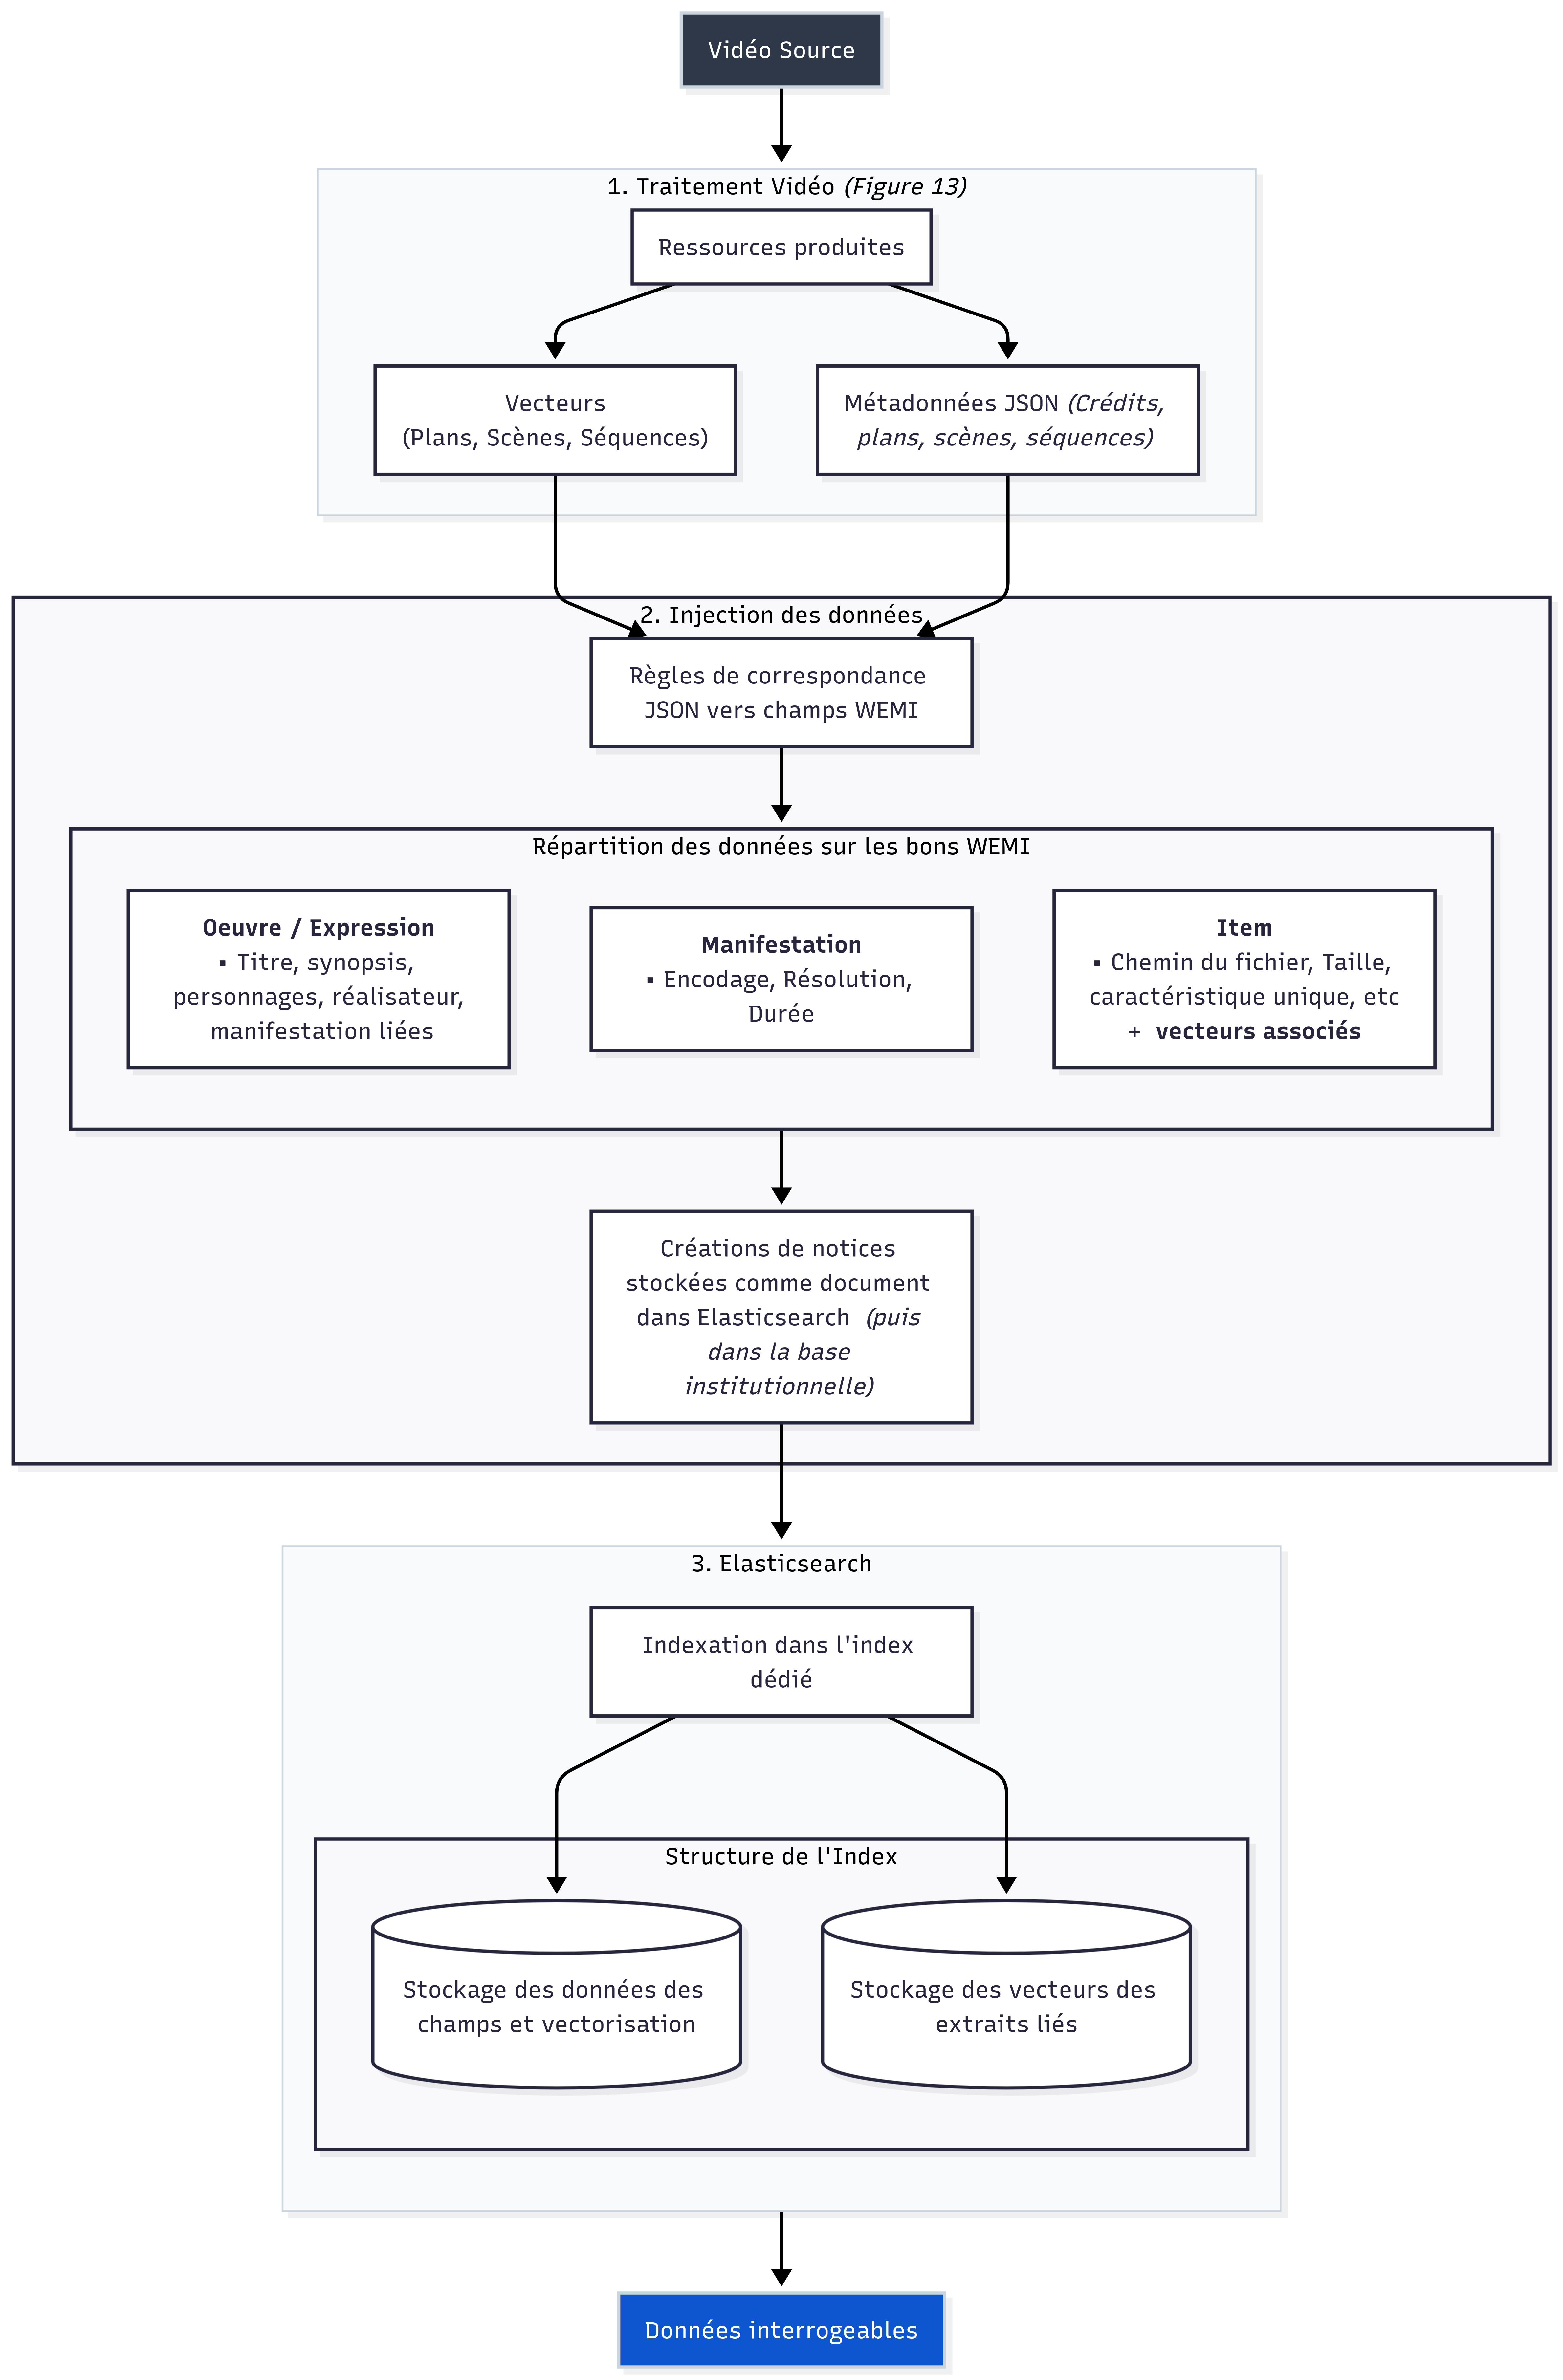
\includegraphics[width=0.8\textwidth]{./Schema/Intégration.png}
	\caption{Schéma du processus d'intégration des données générées par le traitement des \glspl{imgani}.}
	\label{fig:intégration}
\end{figure}

\vspace{0.5cm}

Grâce à la première partie du processus, nous disposons des méta-données à mettre dans les bons champs et niveaux \gls{WEMI} ainsi que des \glspl{vcs} des \glspl{pl}, \glspl{sc} et \glspl{sq} à associé aux notices correspondantes. \newline

Le \coeur de ce processus se situe à notre étape 2. Il s'agit d'assurer l'intégration de ces différentes ressources aux bons endroits applicatifs. Pour les méta-données, il s'agit d'établir des règles de correspondances entre les champs de nos \J et ceux champs de notre index \gls{ES} rattachés aux bons \gls{WEMI}. Grâce à la stabilité du \J et des champs \gls{ES}, on s'assure de la répétabilité de la procédure. 

Pour cela, on établi la structure du \J et la correspondes des champs en amont. Ainsi, on donnera à nos différents outils les \textit{templates} à remplir en fonction de ce qui est attendu. Chaque \textit{template} sera dors et déjà compatible avec les champs \gls{ES} ciblés.

Les \glspl{vcs} étant associé aux \J, ils seront automatiquement rattachés aux bonnes notices \glspl{it}. L'avantage de les stocker dans \gls{ES} est de permettre, par la suite, l'utilisation de la \guillemet{recherche augmentée}. On peut imaginer une utilisation alternative de cette dernière centrée sur la \gls{table} des médias. Une requête basée sur une description d'une action ou d'un thème créer un \gls{vcs} comparable avec ceux des \glspl{pl}, \glspl{sc} et \glspl{sq}. Ce qui permet donc de rechercher des extraits par des requêtes imprécises. 

\subsection{Proposition de conception technique}

Ici, nous allons proposer des outils à utiliser pour ce processus. Notons cependant qu'un tel processus demande des technologie variées. Un effort de réutilisations des mêmes technologies à été menée. Ajoutons que, bien que non estimée, la mobilisation de toutes ces technologies demande des ressources informatiques importantes.\newline

Nous allons prendre chacun de nos deux traitements et présenter les outils à utiliser pour chaque étape en nous concentrant sur leur utilisation dans notre processus.\newline

Commençons par notre processus de traitement\footnote{Voir figure \ref{fig:indexation} page \pageref{fig:indexation}} qui articule au sein d'un script python :

\begin{enumerate}
	
	\item Pour la première étape, nous utilisons PySceneDetect\footnote{Voir \fullref{PyScene}}, FFmpeg\footnote{Voir \fullref{FFmpeg}} et le \gls{VLM} \textit{SmolVLM2-2.2B-Instruct}\footcite{HuggingFaceTBSmolVLM222BInstructHugging2024}. En combinant la détection des ruptures visuelles de PySceneDetect et la manipulation vidéo de FFmpeg, on extrait tous les \glspl{pl}. Avec \textit{SmolVLM2-2.2B-Instruct}, on pourra dès lors lire les crédits et les stocker dans le fichier \J dédié. Nous proposons ce modèle car il est très léger, pesant 2,2 giga octets seulement, tout en étant précis et fiable. 
	
	\item Pour notre seconde étape, l'extraction d'une image clé d'un \gls{pl} et de son extrait audio, FFmpeg l'intègre nativement. C'est une fonction dédiée basée sur la détections des points clés des images et sur la sélection de celles en contenant le plus.
	
	\item Pour notre troisième étape, afin d'identifier et reconnaître les entités, les personnes et l'ambiance sonore nous utilisons 3 outils. SAM2 pour la \gls{seg} et leu suivis des objets\footnote{Voir \fullref{SAM2}}. FaceNet pour la reconnaissance de visages\footnote{Voir \fullref{FaceNet}}. Puis QWEN2-Audio pour l'analyse de la bande son.\footnote{Voir \fullref{QWEN2}}. L'application successive de ces outils, dans un ordre à définir, permet d'identifier les célébrités et d'analyser l'ambiance sonore ainsi que les entités présentes. 
	
	\item Pour notre quatrième étape, celle de \gls{Vecsion} des éléments identifiés, il y a deux approches possibles : 
	
	\subitem L'utilisations de \textit{SmolVLM2-2.2B-Instruct} et QWEN2-Audio pour générer des analyses sémantiques textuelles. Sur ces analyses, nous appliquons notre modèle de \gls{Vecsion} déjà éprouvé \textit{intfloat/multilingual-e5-small}, ou \textit{intfloat/multilingual-e5-base}, pour générer des \gls{vcs}. La problématique se situe dans le fait qu'on génère des \gls{vcs} sur du texte et non à partir de l'image ou du son. Cela implique un intermédiaire pouvant créer un décalage.
	
	\subitem Ou l'utilisation de \gls{mmlts} comme CLIP\footnote{\fullref{clip}} capable d'analyser aussi bien le son que la vidéo. Contrairement aux processus précédent, les \gls{vcs} générés par CLIP à partir des vidéos et sons et non d'analyse textuelles précédemments générées.
	
	\item Pour notre cinquième étape, nous avons recours à une matrice de proximité. C'est une méthode de calcul tabulaire permettant d'établir le degré de similarité entre deux objets à partir de différents éléments. En somme, cela permet d'établir des proximités entre les \glspl{pl} selon leurs \gls{vcs} et leurs horodatages. Ainsi, deux \glspl{pl} à l'horodatage proche seront plus facilement rapproché que deux \glspl{pl} à l'horodatage très éloignés. Cela permet d'éviter de consituer des \glspl{sc} avec des \glspl{pl} éparpillés dans la bande vidéos.
	
	\item Pour la deuxième partie de cette cinquièreme étape, nous utilisons notre \gls{LLM} \textit{Gemma-4-31B}\footnote{Voir \fullref{Gemma}} afin d'analyser tous les \J des \glspl{pl} rassemblé et de constituer un \J pour la \gls{sc}.
	
	\item Pour les séquences et \gls{oe}, aux étapes 6, 6 \guillemet{bis} et 7, nous réitérons ce traitement. En effet, le traitement n'est guère différent si ce n'est qu'on ne l'applique plus aux \glspl{pl} mais aux \glspl{sc}. Cela ne nécessite pas de changement. 
\end{enumerate}

Pour le processus d'intégration des données dans l'application, les technologies sont déjà présente. En effet, pour notre étape numéro 3 sur le stockage et la mise à disposition des données dans \gls{ES}, c'est le logiciel qui s'en charge. Nous n'avons donc pas d'ajout à effectuer.

Cependant, l'étape précédente d'injection des données demande une technologie précise afin de créer les correspondances de champs entre les \J et \gls{ES}. La librairie \textit{Pydantic}, déjà utilisée pour la \textit{recherche augmentée}, permet d'établir et de vérifier ces règles en amont. L'intégration est alors exécuté après validation des fichiers \J. Les \gls{vcs} sont quant à eux déjà pris en charge par un module spécifique d'\gls{ES}.\newline

Ce processus mobilise un grand nombre de technologies différentes, certains sont assez volumineuse même lorsqu'on prend les options \guillemet{légères}. Nous pensons notamment aux \gls{VLM} et \gls{ALM} qui mobilisent énormément de ressources.  

Le poids du processus est donc conséquent. Il s'agit de procéder à énormément de calcul complexes dans une chaîne de traitement iétrative. En effet, elle s'applique sur chaque image clés de chaque \gls{pl} sachant qu'une \gls{oe} cinématographique peut se composer aisément de plus de 1000 images clés. C'est donc un processus long, répétitf et très demandeurs en ressources. Modifier le processsus pour traiter toutes les images clés en lots, et non successivement, ne représente pas une solution. Cela risque de saturer la \gls{RAM} et les capacités des outils conduisant à des hallucinations. 

\subsection{Proposition de conception du parcours utilisateurs}

Nous allons ici procéder à une analyse afin d'identifier les points d'attentions en terme d'\gls{ux} et d'\gls{ui}.\newline

D'abord, le processus présenté est pensé comme étant interne à l'application. Ce qui demande donc de le connecter à des éléments déjà présents afin de ne pas perturber l'utilisateur. C'est ce que nous avons fait avec la \guillemet{recherche augmentée}. Dans SkinSoft l'utilisateur à la possibilité d'intégrer des fichiers dans le logiciel par simple \guillemet{glisser / déposer}. On peut alors penser qu'au moment de déposer une vidéo, l'application genère une fenêtre d'interraction demandant à l'utilisateur de choisir soit une intégration simple, soit l'indexation semi-automatisée.

Il faut établir un choix et message clair, permettant de faire comprendre qu'il ne s'agit de produire automatiquement une indexation mais d'en suggérer une. À ce titre, l'humain garde son rôle de décisionnaire et peu valider, modifier ou invalider la production. Si l'utilisateur choisi l'indexation semi-automatiséen alors le processus décrit s'applique. Cependant, ce processus doit s'appliquer sous contrôle de l'utilisateur. Ce qui demande donc une interface et une expérience d'utilisations.\newline

Cela nous amène à la notion de choix. Notre processus est complexe et prend en charge divers aspects de traitement. La division d'une vidéo à différentes échelles, l'extractions de différentes données et la création de notices \gls{WEMI} pré-remplies. Chacun de ces aspects demande des choix utilisateurs. 

En premier lieu, il se peut qu'un utilisateur ne souhaite pas diviser sa vidéo en unité plus petites notamment car il s'agit déjà d'un extrait. Il faut donc offrir cette possibilité

Ensuite, il se peu que l'utilisateur souhaite créer l'\gls{it} d'un \gls{WEMI} préexistant. Au quel cas, l'analyse des crédits et l'analyse d'éléments appartenants aux niveaux \gls{oe} et \gls{exp} ou \gls{man} ne sont pas nécessaire. 

Enfin, il se peut également qu'un utilisateur souhaite seule compléter des notices préexistantes. Cet usage implique un changement de la fonctionnalité afin qu'elle s'applique sur des éléments préexistants, et des champs déjà remplis.\newline

Chacun de ces cas d'usages place la notion de choix au \coeur de l'\gls{ux} et de l'\gls{ui}. Cela implique que la fonctionnalité doit être hautement modulable afin de répondre à différentes attentes simples comme complexes. Ainsi l'\gls{ux} doit être basée sur la notion de choix et l'\gls{ui} doit présenter une interface permettant à l'utilisateur de moduler la fonction. Cela peut se faire via la sélection ou déselection de certaines options de traitements. \newline

De plus, il faut offire la possibilité de modifier, valider ou invalider le travail effectué à chaque étape de traitement. Par exemple, le découpage en \glspl{pl}, \glspl{sc} ou \glspl{sq} peut ne pas être satisifaisant, ainsi une interface doit permettre de modifier cela simplement. Cela doit aussi être valable pour les données générées dans les \J. Il faut penser à une façon de présenter les informations en retirant l'aspect technique du \J. Cela peut être par une pré-visualisation de la notice créée avec les champs pré-remplis avec les données correspondantes. Les modifications effectuées ici se répliquent ensuite sur le fichier \J.\newline

En somme, l'intégration des questions du parcours utilisateurs, centré sur une approche \textit{human in the loop}, complexifie techniquement le processus. Notamment en imposant divers stade de gestion d'erreur et une modularité du code. 

De plus, le nombre d'éléments à prévoir en terme de validation et d'étape de contrôle demande une interface dédiée. Ce qui amène à complexifier encore le \gls{sgc} par l'ajout d'une fonctionnalité supplémentaire avec sa propre expérience et interface. 

\subsection{Apports et limites}

Le processus que nous avons dépeint met en lumière plusieurs éléments quant à la possibilité de s'appuyer sur des processus semi-automatisé pour traiter de telle typologie. Mais il est important de mettre en lumière l'apport de ces outils, mais aussi leurs limites. L'indexation semi-automatisée est une solution très contrastée, renouvelant des problématique et en créant de nouvelles. 

Ce processus, qui n'a pas encore fait l'objet d'un \textit{proof of concept}, semble ouvrir la voix au traitement automatisée de cette typologie documentaire. Différents outils sont aujourd'hui articulable afin de répondre aux besoins les plus précis de traitement de cette typologie documentaire. Mais ce processus tout à fait conceptuel présente des difficultées majeures. \newline

Ce processus présente deux avantages majeurs. Le premier est la possibilité de traiter des \gls{oe} d'\gls{imgani} de plusieurs heures à la chaîne, et sans interventions humaine. Cela permet de décharger l'utilisateur de l'analyse manuelle de plusieurs heures de bande vidéos, et lui permet de s'occuper d'autres tâches. Le second avantage c'est ça répétabilité. Par la production de \J dans un format fixe et interfacée avec les index \gls{ES} concernés, ce processus est très stable. On s'assure d'extraire les mêmes métadonnées et de les intégrer toujours au même endroit. 

Il faut ajouter à cela qu'il reste simple d'usage. Il suffit d'entrer une \gls{oe}, de laisser le traitement s'accomplir, puis de contrôler à chaque étape afin de rectifier. Le seul défaut, est que la plus part des outils ne peuvent pas faire l'objet d'un \gls{ft}. Prenons l'exemple de PySceneDetect, il s'appuis sur la \gls{CV} algorithmique c'est à dire sans \gls{IA}. Si les détections de changements de plans sont erronnés, la correction manuel par l'utilisateur n'entraîne pas d'améliorations à long terme.

Nous pouvons également dire qu'il reste largement flexible. Par exemple, le modèle SAM2 est parfaitement compatible avec un \gls{mod} YOLO\footnote{Voir \url{https://www.ultralytics.com/fr/yolo} pour plus d'informations} pour la détection et l'identification d'objets précis. Ou bien encore le \gls{mod} FaceNet peut s'entraîner sur une base de données constituée par l'institution pour détecter des personnalités précises. De cette manière, le processus est très souple et offre diverse possibilité d'adaptation intéressante.\newline

Les limites sont également nombreuses. D'abord l'absence de reconnaissance de la typologie de l'\gls{imgani}. En effet, dans ce processus nous n'avons pas incorporer ce principe de détection typologie car nous ignorons l'efficacité de ces technologies à accomplir cette tâche. 

En effet, les \gls{VLM} et \gls{mmlts} sont entraînés pour déterminer et décrire ce qu'il se passe au sein d'une image ou d'une \gls{sc}. Ils peuvent aller plus loin par des analyses colorimétriques, et sonore avec des \gls{ALM}, afin de déterminer le ton du film, le sentiment qui s'en dégage. Cependant, nous n'avons rien trouver au sujet de leurs capacité à distinguer un film muet, d'un film en couleur et sonore, d'un film d'animation. 

Sans que cela semble impossible, aujourd'hui les outils que nous possédons sont trop peu entraînés et spécialisé sur ce domaine. D'autant que la typologie d'un objet patrimonial peut ne pas correspondre à une typologie publique. Ajoutons également que certaines typologie se distingue par des nuances très fines. Par exemple comment distinguer une \gls{imgani} professionnelle d'une \gls{imgani} amateur ? Elle se distingue par les moyens de productions, la possibilité de reconnaître les personnes qui s'y trouvent et la présence d'une construction sémantique de l'\gls{oe}. Mais toutte ces dimensions semblent difficile à être prise en compte.

Ajoutons à cela le fiabilité des métadonnées générées. Concernant la fiabilité, nous en revenons à notre problématique d'hallucination des \gls{mod} d'\glspl{IA} sur lequel nous n'avons que peu de contrôle. Étant au \coeur des données patrimoniales, puisqu'il s'agit de la produire, le contrôle de ce phénomène est important. \newline